\documentclass[conference]{IEEEtran}
\usepackage{amsmath}
\usepackage{afterpage}

\input epsf
\usepackage{graphicx}
% correct bad hyphenation here
\hyphenation{op-tical net-works semi-conduc-tor IEEEtran}
\begin{document}

%+++++++++++++++++++++++++++++++++++++++++++
\title{\LARGE  DeepNeuroPred: Advancing Neuropeptide Classification.}
%+++++++++++++++++++++++++++++++++++++++++++
\author{
    Sarthak Jindal, D Veera Harsha Vardhan Reddy, Avi Vyas, Godavarthi Sai Nikhil
    
}
\maketitle
\begin{abstract}

Neuropeptides, small biologically active molecules found in the nervous systems of all animals, play critical roles in cell-to-cell communication and regulate various physiological processes and behaviors. A new neuropeptide classification model has emerged as a promising tool by integrating convolutional neural networks (CNNs) with global multi-head attention mechanisms to enhance protein sequence representation. Despite its potential, challenges in classification accuracy and model interpretability have limited progress in peptide research and drug discovery. To overcome these limitations, the model was optimized using a larger, updated dataset and transfer learning techniques with the EsmModel architecture. Multi-scale CNN layers were employed for local feature extraction, while global multi-head attention captured sequence-wise dependencies. Key contributions included the development of a novel model, DeepNeuroPred, enhanced data preprocessing techniques, and refined regularization methods. By integrating transformer-based protein language models (PLMs) and additional feature encodings, the model achieved significant improvements in accuracy, robustness, and interpretability. These advancements provide a state-of-the-art tool for neuropeptide identification, supporting neural communication research and the development of treatments for neurological disorders.

\end{abstract}

\IEEEoverridecommandlockouts

\begin{keywords}
Neuropeptides, Convolutional neural networks (CNNs), Transformer, Classification.
\end{keywords}

\IEEEpeerreviewmaketitle

\section{Introduction}

Neuropeptides are small biologically active molecules found in the nervous systems of all animals, including humans. These molecules act as critical signaling agents, facilitating cell-to-cell communication and regulating a diverse range of physiological processes such as \textbf{metabolism}, \textbf{reproduction}, \textbf{stress response}, and \textbf{behavior}. Their role in neural communication and disease mechanisms makes them valuable \textbf{biomarkers} and \textbf{therapeutic targets} for diagnosing and treating conditions like \textbf{depression}, \textbf{diabetes}, \textbf{cardiovascular diseases}, and \textbf{neurological disorders}.

Traditionally, neuropeptides have been identified through experimental methods like \textbf{mass spectrometry} and \textbf{liquid chromatography}, which are precise but time-intensive and resource-heavy. Computational approaches have emerged as cost-effective alternatives, but early machine learning models depended heavily on manually curated features and motifs, limiting their ability to generalize. Although deep learning models can capture intricate sequence patterns, challenges such as the need for large annotated datasets and the lack of \textbf{model interpretability} still limit their broader use.

To address these limitations, this research introduces \textbf{DeepNeuroPred}, a novel neuropeptide classification model that combines advanced deep learning techniques with improvements in \textbf{protein language modeling}. Built on the \textbf{Evolutionary Scale Modeling (ESM)} architecture, DeepNeuroPred applies transfer learning to generate semantic representations of protein sequences. \textbf{Convolutional neural network (CNN)} layers are used to extract local features, while \textbf{multi-head attention mechanisms} capture long-range dependencies, improving both classification accuracy and \textbf{interpretability}. Additional improvements, such as data preprocessing, attention score visualization, and regularization techniques, ensure the model is both \textbf{reliable} and \textbf{transparent}.

The motivation for this work comes from the increasing demand for accurate and interpretable neuropeptide classification tools to advance bioinformatics and \textbf{drug discovery}. By addressing gaps in performance and interpretability, \textbf{DeepNeuroPred} represents a significant step forward in peptide research, enabling the identification of novel neuropeptides and accelerating the development of \textbf{targeted therapies} for \textbf{neurological disorders}. This model aims to balance computational efficiency with biological interpretability, contributing to practical solutions in the biomedical field.

\section{Description of the Problem}

The classification of neuropeptides from protein sequences remains a complex challenge in computational biology. Neuropeptides are essential for regulating vital physiological processes such as metabolism, stress response, and behavior. Accurately identifying these molecules is essential for advancing neurobiology research and drug discovery. However, traditional experimental methods like mass spectrometry and liquid chromatography are resource-intensive, time-consuming, and not scalable for large datasets.

Existing computational models, such as \textbf{PredNeuroP} and \textbf{NeuroPred-FRL}, have made progress in classifying neuropeptides but still face significant limitations. These models struggle to capture the intricate dependencies and sequence patterns inherent in neuropeptides. Many also lack sufficient interpretability, making it difficult for researchers to understand how specific classifications are made. The reliance on manually curated features or shallow models also restricts generalizability, hindering their application to large and diverse datasets.

A key challenge in neuropeptide classification is effectively modeling long-range dependencies within protein sequences, as well as ensuring transparency in the model's decision-making process. This research addresses these challenges with \textbf{DeepNeuroPred}, which leverages advanced deep learning techniques like protein language modeling and multi-head attention to capture both local and global sequence patterns. Moreover, attention-based visualizations ensure interpretability, providing a reliable and transparent solution for classifying neuropeptides. This approach not only improves classification accuracy but also supports the discovery of novel neuropeptides, which is essential for the development of targeted therapies.

\begin{table*}[ht]
\centering
\caption{Summary of Computational Methods for Neuropeptide Classification}
\begin{tabular}{|p{2.5cm}|p{3.5cm}|p{3.5cm}|p{3.5cm}|p{2.5cm}|}
\hline
\textbf{Model} & \textbf{Approach} & \textbf{Strengths} & \textbf{Limitations} & \textbf{References} \\
\hline
Motif-based Search & Sequence alignment, motif recognition & Simple, interpretable & Low sensitivity, limited scalability & Meydan et al. (2013) \cite{meydan2013} \\
\hline
CNN-based Methods & Convolutional layers for feature extraction & Improved local feature extraction & Limited global context capture & Li et al. (2008) \cite{li2008} \\
\hline
SVM and ML-based Models & Machine learning with feature engineering & Good for small datasets & Requires manual feature selection & Salam et al. (2024) \cite{salam2024} \\
\hline
LSTM-based Models & Recurrent neural networks for sequence dependencies & Captures long-range dependencies & Sequential data processing limitations & Yi et al. (2019) \cite{yi2019} \\
\hline
Transformer-based Models & Attention mechanisms for global context & Captures long-range dependencies effectively & Model interpretability challenges & Rives et al. (2021) \cite{rives2021} \\
\hline
Transfer Learning-based Models & Pre-trained protein language models & Generalizes across diverse datasets & Requires large computational resources & Elnaggar et al. (2021) \cite{elnaggar2021} \\
\hline
\end{tabular}
\end{table*}

\section{Literature Review}

Neuropeptides play a central role in neural communication and have diverse physiological functions across species. Accurate classification of neuropeptides from protein sequences is a crucial task in bioinformatics. The complexity of neuropeptide sequences presents significant challenges to traditional classification methods, necessitating advanced machine learning approaches for improved accuracy and interpretability. In recent years, several models have been developed, each employing different techniques to enhance the accuracy and efficiency of neuropeptide classification. This section reviews key advancements in the field, focusing on computational methods and deep learning architectures that have been applied to neuropeptide classification.

\subsection{Traditional Approaches to Neuropeptide classification} Early methods of neuropeptide classification relied heavily on sequence alignment techniques and motif-based searches. These approaches, such as those discussed by \cite{meydan2013}, were limited by the complexity and variability of neuropeptide sequences across species. Motif-based approaches aimed to identify conserved patterns within protein sequences that are characteristic of neuropeptides, but these techniques often struggled with low sensitivity and specificity, especially for peptides that did not adhere to clear sequence motifs. Additionally, the rapid expansion of peptide datasets posed further challenges, as traditional methods were ill-equipped to handle large-scale data.

\subsection{Machine Learning-Based Methods} To overcome the limitations of traditional approaches, machine learning models have been increasingly applied to neuropeptide classification. \cite{salam2024} proposed the use of support vector machines (SVMs) and other machine learning techniques to classify bioactive peptides. However, these models required extensive feature engineering and struggled with capturing complex sequence dependencies.

Subsequently, the field moved towards more advanced methods, such as the NeuroPred model, which utilized convolutional neural networks (CNNs) to improve the classification of neuropeptides. \cite{li2008} introduced a CNN-based approach that focused on learning hierarchical features from peptide sequences. While this method improved classification performance over traditional techniques, it still faced challenges in generalizing across diverse peptide families and integrating global sequence information.

\subsection{Deep Learning and Transformer-Based Models} The introduction of deep learning architectures, such as recurrent neural networks (RNNs) and long short-term memory (LSTM) networks, enabled further improvements in peptide classification. \cite{yi2019} employed LSTMs to capture long-range dependencies in peptide sequences, offering better performance than earlier models. However, these models were still limited by their reliance on sequential data processing, which made it difficult to capture global patterns in large datasets.

Recent advancements in transformer-based architectures, such as BERT and its variants, have significantly improved protein sequence modeling. Transformers, which rely on attention mechanisms, allow for better representation of long-range dependencies in sequences. Notably, the NeuroPred-PLM model combined convolutional layers with global multi-head attention, providing state-of-the-art results in neuropeptide classification \cite{rives2021}. This architecture effectively integrates local and global information, allowing the model to capture both fine-grained features and long-distance dependencies. Additionally, the use of pre-trained protein language models (PLMs) has led to improvements in feature extraction from biological sequences, as demonstrated by \cite{rives2021}.

\subsection{Challenges and Opportunities in Neuropeptide classification} While deep learning models such as CNNs, LSTMs, and transformers have shown great promise, challenges remain. One key issue is the interpretability of these models. Many of the current architectures function as "black boxes," making it difficult for researchers to understand how the model arrives at its classification. Additionally, there is still a need for models to handle the vast diversity in neuropeptide structures and functions. The integration of transfer learning, as explored by \cite{elnaggar2021}, presents an opportunity to address these challenges by enabling models to generalize across different datasets.

Further developments in neuropeptide classification, such as the proposed iNP\_ESM model, aim to enhance accuracy while improving model transparency and interpretability. The model's use of advanced data preprocessing, visualization techniques, and refined regularization methods represents a promising step forward in addressing the current limitations of neuropeptide classification technologies \cite{li2024}.



% \begin{figure*}[htbp]
%     \centering
%     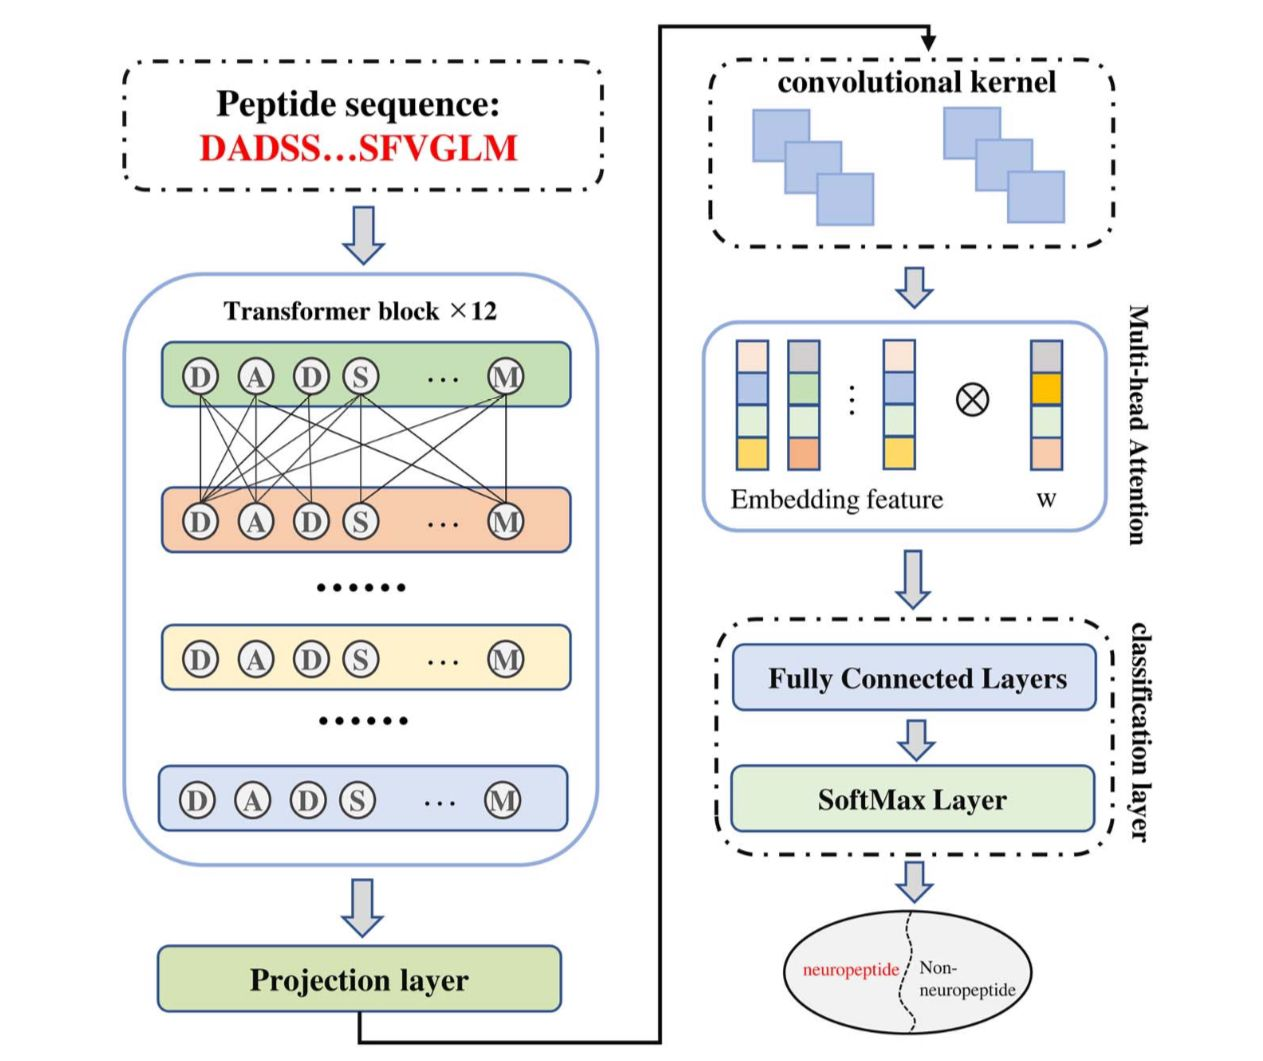
\includegraphics[width=0.7\textwidth,height=9cm]{1.jpg} % replace with the image file path
%     \caption{The flowchart of the model architecture.}
%     \label{fig:model_architecture}
% \end{figure*}


\section{Methodology}

This research utilized deep learning methodologies for \textbf{neuropeptide sequence classification}. The approach involved processing a curated dataset of positive (neuropeptide) and negative (non-neuropeptide) sequences to build a robust classification model. A \textbf{Transformer-based model} was utilized to enhance classification accuracy and address challenges in identifying neuropeptides from protein sequences.

The methodology was divided into several key stages: \textbf{data collection}, \textbf{data preprocessing}, \textbf{model architecture design}, \textbf{model training}, and \textbf{performance evaluation}. The model leveraged the capability of Transformers to capture both local and global dependencies in protein sequences, providing a robust framework for neuropeptide classification.

\subsection*{A. Dataset}

Data was sourced directly from the \textbf{NeuroPred-FRL} website, providing an updated version that included \textbf{2,929 new sequences}, resulting in a total of \textbf{5,214 neuropeptide} and \textbf{6,641 non-neuropeptide} sequences. The raw dataset was organized into four files: two training files (one for positive and one for negative sequences) and two testing files (also divided into positive and negative). These files were combined, and random shuffling was applied to ensure a more generalized dataset for subsequent training and evaluation.

\vspace{-1em}

\begin{figure}[h]
    \centering
    % 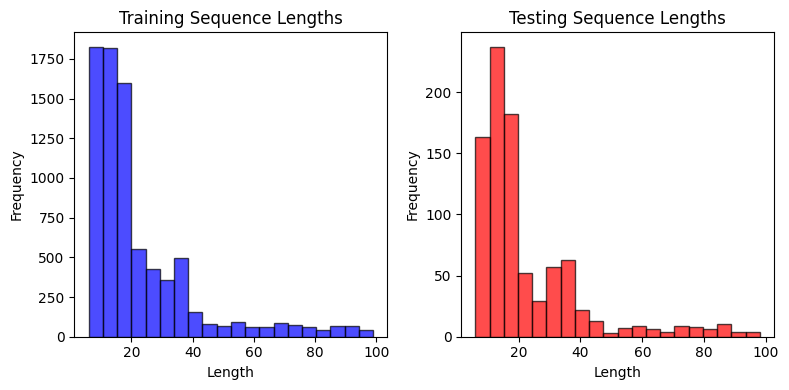
\includegraphics[width=1 \linewidth]{Images/1.png}
    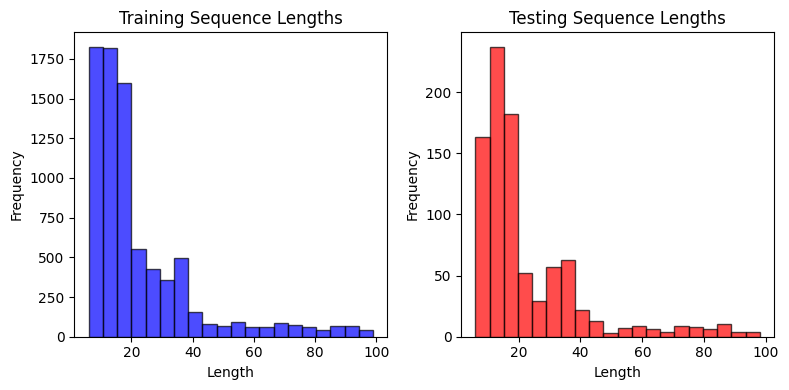
\includegraphics[height = 5cm, width=9cm]{Images/1.png}
    \vspace{-1.6em}
    \caption{Visualization of sequence class distribution in the dataset.}
    \label{fig:seq_distribution}
\end{figure}

Figure \ref{fig:seq_distribution} illustrates the distribution of neuropeptide and non-neuropeptide sequences across the dataset, highlighting the balance between positive and negative classes. This balance is critical to ensuring unbiased performance metrics during model validation.


\subsection*{B. Data Preprocessing}

The sequence data was prepared using the \textbf{AutoTokenizer} from the pre-trained \textbf{facebook/esm2\_t33\_650M\_UR50D} model. This tokenizer applied padding and truncation to standardize each input to a uniform length of \textbf{128 tokens}, converting training and testing sequences into a suitable format for the model. The training and testing labels were extracted and converted into tensors for efficient processing during model training and evaluation. This stage was essential for structuring the raw sequence data for deep learning applications.

\subsection*{C. Model Architecture}
The model architecture presented in this research is designed to predict neuropeptide sequences effectively \cite{wang2023}. It is based on a deep learning framework that incorporates advanced techniques such as \textbf{embedding layers}, \textbf{Transformer encoder layers}, \textbf{convolutional layers}, \textbf{multi-head attention mechanisms}, and \textbf{fully connected layers}. These components work collaboratively to extract meaningful features from the sequence data and perform accurate classification tasks.

\vspace{-1.4em}
    
\begin{figure}[h]
    \centering
    % 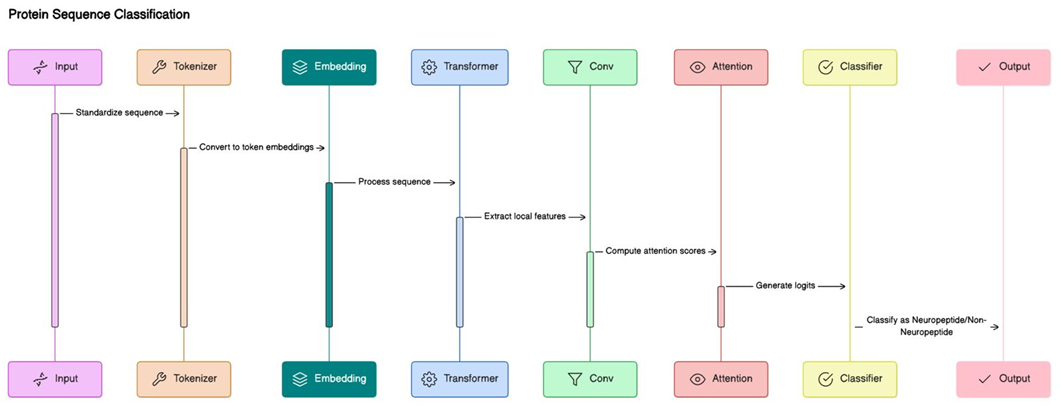
\includegraphics[width=1\linewidth]{Images/2.png}
    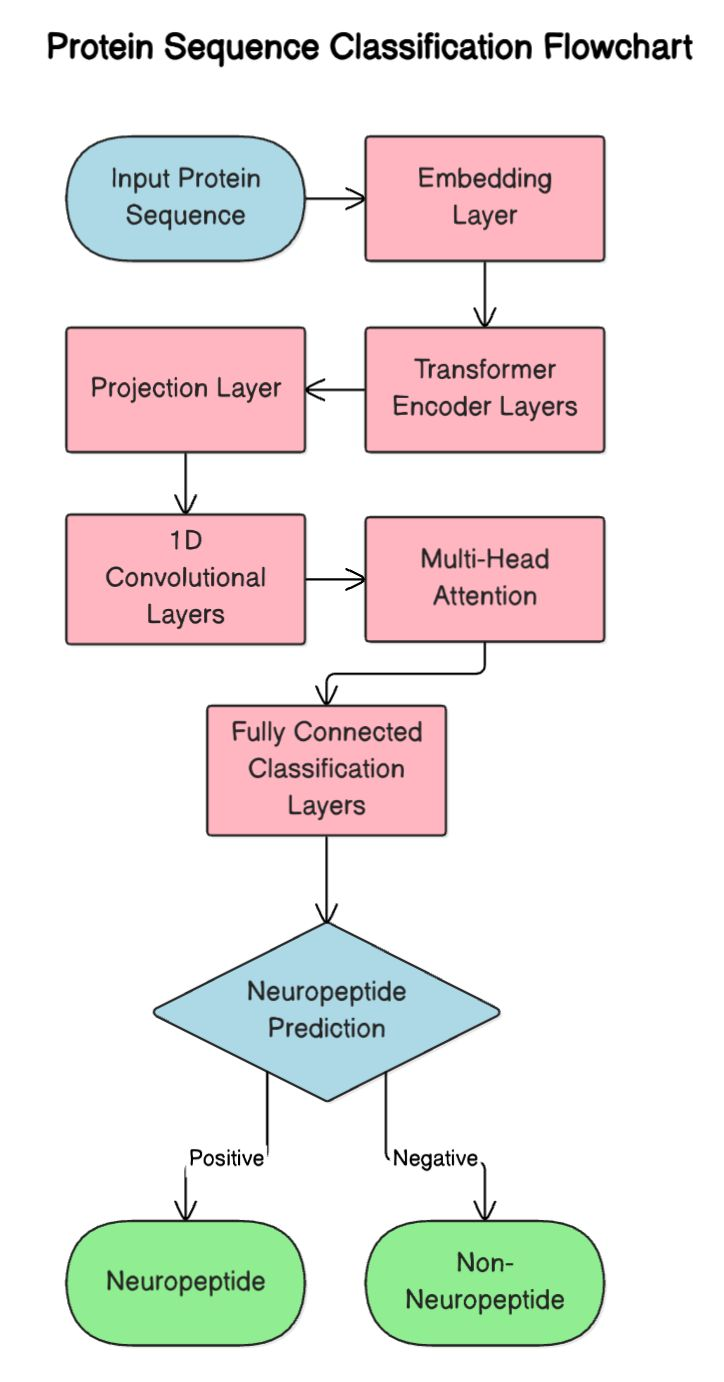
\includegraphics[height=15 cm,width=9.5cm]{Images/3.jpg}
    \vspace{-1.6em}
    \caption{Overview of the protein sequence classification process.}
    \label{fig:overview}
\end{figure}

Figure \ref{fig:overview} provides a detailed overview of the protein sequence classification process, starting with a \textbf{tokenizer} for preprocessing and an \textbf{embedding layer} for numerical feature representation. \textbf{Transformer encoders} capture sequence dependencies, \textbf{1D convolution} extracts local patterns, and \textbf{multi-head attention mechanisms} model complex interactions. Finally, a \textbf{classifier} classifies neuropeptide sequences, ensuring robust and accurate results.

\subsection*{1) Feature Extraction from the DeepProtein Model}
Feature extraction transformed raw input sequences into meaningful representations through several processing layers. The embedding layer first converted token IDs into dense vector representations, facilitating a richer understanding of the input data. The subsequent Transformer encoder layers further refined these representations by applying self-attention mechanisms, enabling the model to focus on relevant parts of the sequence.

\vspace{-1em}
\begin{figure}[h]
    \centering
    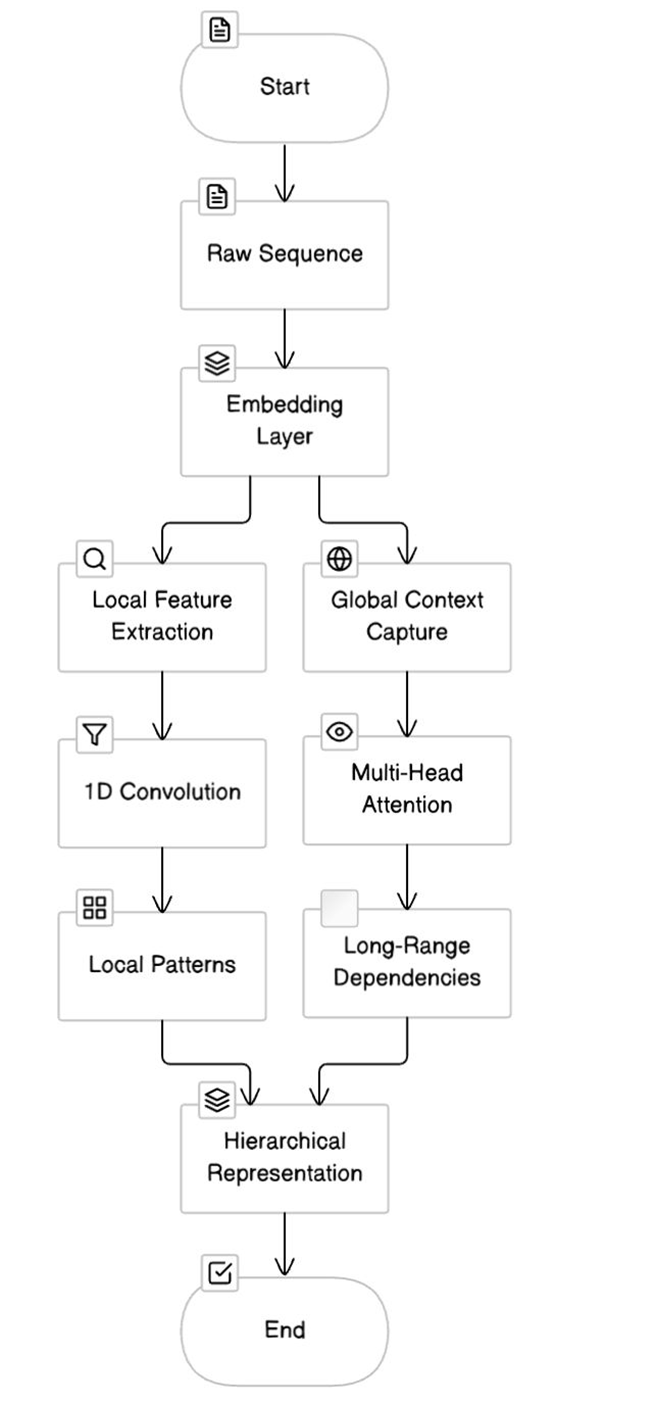
\includegraphics[height = 14.8cm, width=10.2 cm]{Images/4.png}
    \vspace{-1.6em}
    \caption{Neuropeptide Feature Extraction Techniques.}
    \label{fig:neuropeptide-feature-extraction}
\end{figure}

Figure \ref{fig:neuropeptide-feature-extraction} illustrates key techniques for neuropeptide feature extraction, including 1D convolution for local pattern detection and multi-head attention for capturing long-range dependencies. Together, these methods enhance the model's ability to generate robust representations and improve classification performance.

\subsection*{2) Model Layers}
\textbf{Transformer Block}

The model contained \textbf{six transformer encoder layers}, each responsible for processing sequential data. Transformers were chosen for their capacity to capture long-range dependencies, which are crucial for biological data. Within each transformer layer, the self-attention mechanism played a crucial role by computing attention scores that determined the focus on different parts of the input sequence. This mechanism allowed the model to dynamically weigh the importance of different tokens, enhancing its ability to capture contextual dependencies. Mathematically, this can be represented as:
\begin{equation}
\text{Attention}(Q, K, V) = \text{softmax}\left(\frac{QK^T}{\sqrt{d_k}}\right) V
\end{equation}
Where \(Q\), \(K\), and \(V\) represent the query, key, and value matrices, and \(d_k\) denotes the dimensionality of the key vectors. Linear transformations were applied within each transformer block to project the input data into a space suitable for attention calculations, allowing the model to learn complex representations through weight adjustments during training. Layer normalization and dropout were also employed to stabilize and accelerate training, as well as to prevent overfitting. 

\vspace{-1em}
\begin{figure}[h]
    \centering
    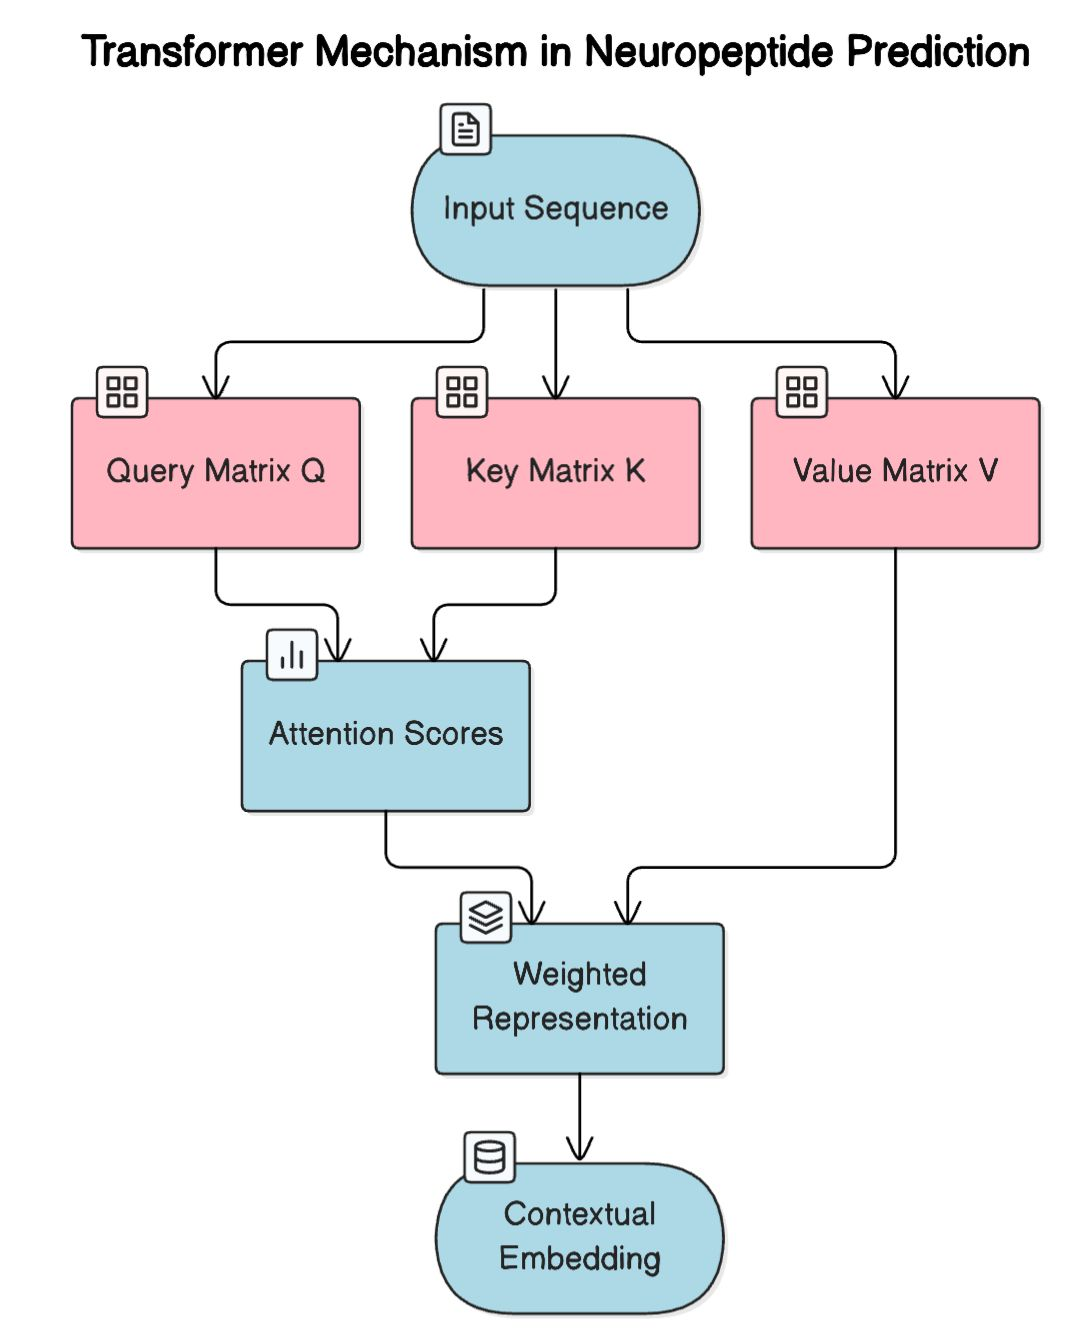
\includegraphics[height = 10.8cm, width=9cm]{Images/5.jpg}
    \vspace{-1.6em}
    \caption{Transformer mechanism used in neuropeptide classification models.}
    \label{fig:transformer-mechanism}
\end{figure}

Image \ref{fig:transformer-mechanism} illustrates the transformer mechanism used in neuropeptide classification models. It shows how an input sequence undergoes transformation through query, key, and value matrices, computing attention scores which are then used to generate a weighted representation of the sequence.


The transformer layer’s structure can be described as:
\begin{equation}
X^{(i)} = \text{TransformerEncoderLayer}^{(i)}(X^{(i-1)})
\end{equation}
where \(X^{(0)}\) is initialized with the embedding output, and \(X^{(N)}\) is the final output of the transformer layers.

\vspace{0.15cm} 
\textbf{Projection Layer}

The projection layer reduced the dimensionality of the transformer layer outputs, enabling more efficient handling of data in subsequent stages. The transformation in the projection layer was given by:
\begin{equation}
P = X^{(N)} W_p + b_p
\end{equation}
where \(W_p\) and \(b_p\) represent the projection weight matrix and bias term, respectively.

\vspace{0.15cm} 
\textbf{Convolutional Layers}

Two 1D convolutional layers followed the projection layer to further refine the features. The first convolution used a kernel size of \textbf{3} to capture local patterns, and the second convolution, with a kernel size of \textbf{1}, reduced the dimensionality while preserving crucial features. ReLU activations introduced non-linearity. This can be expressed as:
\begin{equation}
C_1 = \text{ReLU}(\text{Conv1D}(P))
\end{equation}
\begin{equation}
C_2 = \text{ReLU}(\text{Conv1D}(C_1))
\end{equation}
Where \(C_1\) and \(C_2\) represent the intermediate representations capturing hierarchical features within the sequence.

\vspace{0.15cm} 
\textbf{Multi-Head Attention}

It was applied to enable the focus on various parts of the input sequence simultaneously. Each attention head computed attention scores based on the learned weight matrix \(W\), with the attention calculation represented as:
\begin{equation}
A = \text{softmax}(C_2 \cdot W^T)
\end{equation}
This allowed the model to weigh the importance of different features, resulting in the overall learned representations.

\vspace{0.15cm} 
\textbf{Classification Layers}

The final representation from the attention mechanism was fed into fully connected layers for classification. The representation was first processed through a ReLU activation function, followed by linear transformations to produce the logits for classification. The softmax function was then used to interpret these logits as class probabilities, as represented by:
\begin{equation}
\hat{y} = \text{softmax}(F_2)
\end{equation}
This output indicated the probability distribution over the classes, with the highest probability indicating the classified class.

\vspace{0.15cm} 
\textbf{Total Trainable Parameters}

The model contained approximately \textbf{23,72,096 trainable parameters}. The extensive use of linear transformations enabled efficient learning of complex mappings between input features and output classes, maintaining flexibility in capturing intricate relationships.

\subsection*{D. Loss Function and Optimizer}
During training, the model utilized \textbf{cross-entropy loss} to evaluate the discrepancy between the classified logits and true labels. This loss function was defined as:
\begin{equation}
L = - \frac{1}{N} \sum_{i=1}^{N} y_i \log(\hat{y}_i)
\end{equation}
Where \(y_i\) and \(\hat{y}_i\) represent the true label and the classified probability for each sample.

The \textbf{Adam optimizer} was chosen for updating the model’s parameters, offering efficient training through its adaptive learning rates and momentum, ensuring faster convergence.

\subsection*{E. Performance Metrics}
Various metrics assessed the model's classification performance, including \textbf{accuracy (ACC)}, \textbf{F1 score (F1)}, \textbf{precision (Pre)}, and \textbf{recall (Rec)}. These metrics provided a comprehensive evaluation of the model's ability to accurately classify sequences, reflecting its overall effectiveness in neuropeptide classification. The corresponding formulas are:
\begin{equation}
\text{Pre} = \frac{TP}{TP + FP}
\end{equation}
\begin{equation}
\text{Rec} = \frac{TP}{TP + FN}
\end{equation}
\begin{equation}
F1 = \frac{2 \cdot (\text{Pre} \cdot \text{Rec})}{\text{Pre} + \text{Rec}}
\end{equation}
\begin{equation}
ACC = \frac{TP + TN}{TP + TN + FP + FN}
\end{equation}
where \(TP\), \(TN\), \(FP\), and \(FN\) denote the numbers of true positive, true negative, false positive, and false negative samples, respectively.

\section{Proposed Improvements and Ideas}

Here are some ideas to develop a new classification model, aimed at improving accuracy, efficiency, and generalization:

\subsection*{A. Utilization of an Updated Dataset} 
The dataset has been updated with an additional \textbf{2,929 sequences}, increasing the diversity and volume of samples. This augmentation is designed to improve generalization and robustness by exposing the classification model to a broader spectrum of neuropeptide and non-neuropeptide sequences. The enhanced dataset ensures the model can reliably distinguish between these classes in diverse biological contexts.

\subsection*{B. Implementation of Tokenization}
The \textbf{AutoTokenizer} from the pre-trained \textbf{facebook/esm2\_t33\_650M\_UR50D} model is applied for tokenization, standardizing all input sequences to a uniform length of \textbf{128 tokens}. This preprocessing step facilitates consistent feature representation and compatibility with the transformer-based architecture, improving classification performance by enabling efficient data processing.

\subsection*{C. Development of a New Model Architecture}
A novel classification model, named \textbf{DeepNeuroPred}, is being developed to address the limitations of existing approaches. The architecture integrates a fine-tuned transformer encoder, optimized convolutional layers for local pattern extraction, and a fully connected classification head for accurate sequence categorization. This design is intended to capture intricate relationships within sequence data while maintaining high interpretability and classification accuracy.

\subsection*{D. Incorporation of Advanced Regularization Techniques}
Advanced regularization techniques are incorporated into the model to reduce overfitting and enhance generalization. These include \textbf{dropout}, \textbf{layer normalization}, and \textbf{weight decay}. Such methods balance model complexity with performance, ensuring the classifier performs reliably on unseen data without compromising its classification accuarcy.

\subsection*{E. Optimization for Computational Efficiency}
To make the model more resource-efficient, optimizations are proposed to reduce computational load while preserving classification accuracy. These include minimizing the number of transformer layers, streamlining convolutional operations, and employing lightweight attention mechanisms. Such modifications improve the model’s accessibility for environments with constrained computational resources while maintaining its efficacy in distinguishing neuropeptide sequences from non-neuropeptide sequences.

\section{Results and Discussion}

This section provides a comprehensive evaluation of the \textbf{DeepNeuroPred} model by presenting its performance across various metrics, graphical analyses, and comparisons. The results are discussed under several categories to highlight the model's robustness, effectiveness, and areas of improvement.

\subsection{Model Training and Testing Performance Analysis}

\textbf{Training and Testing Metrics:} The \textbf{DeepNeuroPred} model achieves consistently high accuracy across both the training and testing phases, demonstrating its effectiveness in classifying neuropeptide sequences. Table~\ref{table:train_test_report} summarizes the key classification metrics \textit{accuracy}, \textit{precision}, \textit{recall}, and \textit{F1-score} for both phases. The close alignment of these metrics between training and testing highlights the model's robustness and generalizability. In particular, the testing phase achieves an accuracy of 87.95\%, with precision, recall, and F1-score maintaining similar levels, indicating minimal overfitting and strong predictive power.

\begin{table}[h]
\centering
\label{table:train_test_report}
\renewcommand{\arraystretch}{1.3}
\begin{tabular}{lcccc}
\hline
\textbf{Metric} & \textbf{Training Phase} & \textbf{Testing Phase} \\ \hline
Accuracy        & 88.00\%                 & 87.95\%                \\
F1-Score        & 88.00\%                 & 87.95\%                \\
Precision       & 88.00\%                 & 88.01\%                \\
Recall          & 88.00\%                 & 87.95\%                \\ \hline
\end{tabular}
\vspace{.6em}
\caption{Classification Metrics for Training and Testing Phases}
\vspace{-2.5em}
\end{table}

\textbf{Confusion Matrix:} The confusion matrix 
(Figure~\ref{fig:confusion_matrix}) for the testing phase provides detailed insights into the model's predictions. For class 0 (non-neuropeptide sequences), the model correctly predicted 382 true negatives and 62 false positives. For class 1 (neuropeptide sequences), it correctly predicted 399 true positives and 45 false negatives. This indicates a balanced performance with more correct predictions than errors, highlighting the model's effectiveness in distinguishing between the classes.


\vspace{-.6em}
\begin{figure}[h]
    \centering
    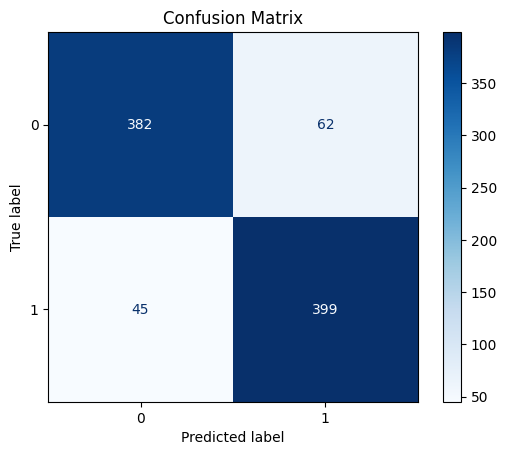
\includegraphics[width=7.5cm, height =7.5cm]{Images/6.png}
    \vspace{-.6em}
    \caption{Confusion Matrix}
    \label{fig:confusion_matrix}
\end{figure}

\textbf{Loss and Validation Accuracy:} The training curves in Figure~\ref{fig:training_curves} illustrate the progression of loss and validation accuracy over the training epochs. The loss consistently decreases, while the validation accuracy steadily increases, signifying effective learning. The absence of significant divergence between training and validation curves suggests minimal overfitting, further demonstrating the model's stability.
\vspace{-.6em}
\begin{figure}[h]
\centering
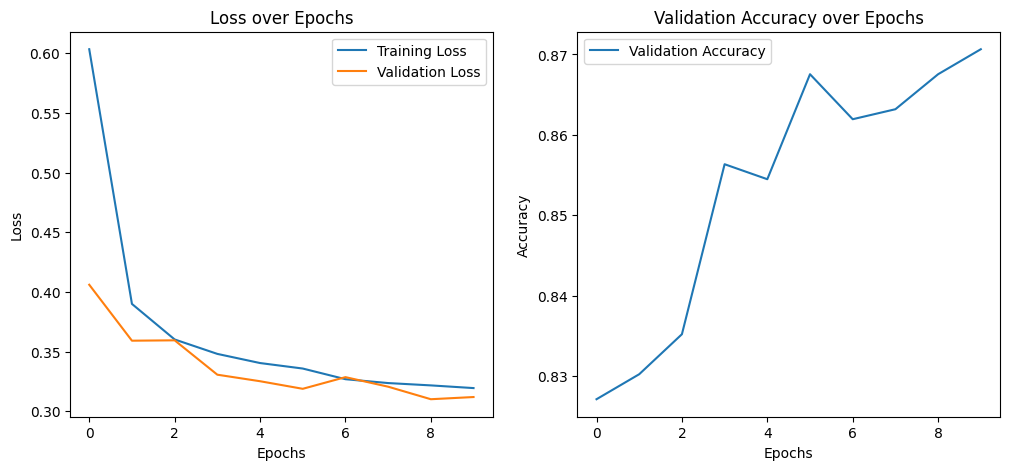
\includegraphics[width=0.9\linewidth]{Images/7.png}
\vspace{-.3em}
\caption{Training Loss and Validation Accuracy over Epochs}
\label{fig:training_curves}
\end{figure}

\textbf{ROC Curve:} The ROC curve (Figure~\ref{fig:roc_curve}) highlights the model's capability to differentiate between neuropeptide and non-neuropeptide sequences. With an area under the curve (AUC) score of 0.93, the model demonstrates a strong ability to correctly classify instances across various threshold settings, indicating excellent classification performance.

\begin{figure}[h]
\centering
\vspace{-.6em}
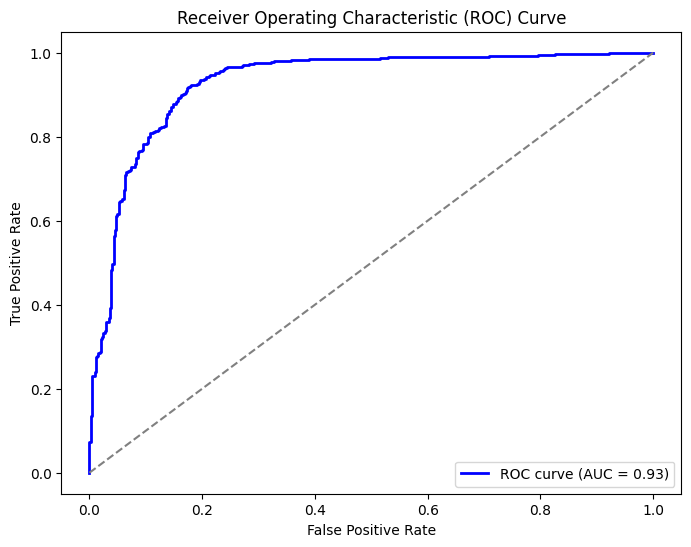
\includegraphics[width=0.8\linewidth]{Images/8.png}
\vspace{-.3em}
\caption{ROC Curve of \textbf{DeepNeuroPred}}
\label{fig:roc_curve}
\end{figure}

\subsection{Hyperparameters Tuning and Cross-Validation}

\textbf{Hyperparameters Tuning:}  
Hyperparameter tuning is an essential process in Deep learning where we systematically search for the best combination of hyperparameters that maximizes model performance. Hyperparameters are configuration settings that control the training process and architecture of the model, such as the learning rate, hidden size, number of attention heads, and the number of layers in a neural network. By exploring different combinations of these hyperparameters, we aim to improve the model's ability to generalize and achieve higher performance metrics, such as accuracy, precision, and recall.

\begin{table}[h]
\centering
\renewcommand{\arraystretch}{1.5}
\resizebox{\linewidth}{!}{%
\begin{tabular}{|c|c|c|c|c|c|c|}
\hline
\textbf{Hidden} & \textbf{Num.} & \textbf{Num.} & \textbf{Learning} & \textbf{Accuracy} & \textbf{Precision} & \textbf{Recall} \\ 
\textbf{Size} & \textbf{Heads} & \textbf{Layers} & \textbf{Rate} & \textbf{(\%)} & \textbf{(\%)} & \textbf{(\%)} \\ \hline
128 & 16 & 4 & 0.0001 & 88.74 & 90.12 & 86.05 \\ \hline
256 & 4 & 4 & 0.0001 & 88.56 & 85.12 & 92.38 \\ \hline
64 & 16 & 4 & 0.0001 & 88.50 & 86.77 & 89.79 \\ \hline
64 & 4 & 4 & 0.0001 & 87.44 & 84.21 & 90.96 \\ \hline
64 & 16 & 6 & 0.0001 & 87.13 & 84.36 & 89.92 \\ \hline
256 & 8 & 4 & 1e-05 & 86.94 & 85.25 & 88.11 \\ \hline
128 & 8 & 4 & 0.0001 & 86.75 & 84.84 & 88.24 \\ \hline
128 & 8 & 6 & 0.0001 & 86.75 & 88.90 & 82.82 \\ \hline
256 & 4 & 6 & 1e-05 & 86.50 & 82.80 & 90.83 \\ \hline
64 & 8 & 4 & 0.0001 & 86.32 & 81.05 & 93.41 \\ \hline
\end{tabular}%
}
\vspace{.6em}
\caption{Top Hyperparameter Configurations During Tuning}
\label{table:hyperparams}
\end{table}

\vspace{-1.5em}
In this study, hyperparameter tuning was conducted to identify the optimal configuration for the model. We evaluated a range of hyperparameters and assessed each configuration based on its performance across multiple metrics. The results presented in Table~\ref{table:hyperparams} show the top 10 configurations, with each row representing a unique combination of hyperparameters. The configurations were evaluated using key performance metrics, including accuracy, precision, and recall. This process is crucial because even small changes in hyperparameters can lead to significant improvements or degradation in model performance. The goal is to find the right balance of hyperparameters that ensures the model performs optimally.

\vspace{.2em}
\textbf{Cross-Validation:}  
Cross-validation is a technique used to evaluate the model’s ability to generalize to unseen data by partitioning the dataset into multiple subsets, or folds. The model is trained on a combination of the subsets and tested on the remaining fold. This process is repeated for each fold, ensuring that each data point is used for both training and testing, leading to a more reliable assessment of the model's performance. In our study, we performed 10-fold cross-validation to ensure robust evaluation of the model across different data subsets.


\begin{table}[h]
\centering
\renewcommand{\arraystretch}{1.4}
\resizebox{\linewidth}{!}{%
\begin{tabular}{|c|c|c|c|c|}
\hline
\textbf{Fold} & \textbf{Accuracy (\%)} & \textbf{Precision (\%)} & \textbf{Recall (\%)} & \textbf{F1-Score (\%)} \\ \hline
1             & 85.07                 & 85.08                  & 85.07               & 85.05                  \\ \hline
2             & 86.69                 & 86.99                  & 86.69               & 86.64                  \\ \hline
3             & 83.21                 & 85.33                  & 83.21               & 82.93                  \\ \hline
4             & 85.32                 & 85.99                  & 85.32               & 85.30                  \\ \hline
5             & 83.71                 & 83.81                  & 83.71               & 83.69                  \\ \hline
6             & 86.94                 & 87.01                  & 86.94               & 86.92                  \\ \hline
7             & 84.83                 & 84.85                  & 84.83               & 84.82                  \\ \hline
8             & 82.96                 & 82.97                  & 82.96               & 82.96                  \\ \hline
9             & 85.18                 & 86.02                  & 85.18               & 85.13                  \\ \hline
10            & 86.80                 & 86.88                  & 86.80               & 86.77                  \\ \hline
\textbf{Avg.} & \textbf{85.07}        & \textbf{85.49}         & \textbf{85.07}      & \textbf{85.02}         \\ \hline
\end{tabular}%
}
\vspace{.6em}
\caption{10-Fold Cross-Validation Results}
\label{table:cross_val}
\end{table}
\vspace{-1.5em}

The results from cross-validation provide a more accurate estimate of model performance, especially when the dataset is limited. The variation in accuracy, precision, recall, and F1-score across different folds is shown in Table~\ref{table:cross_val}. This table demonstrates the consistency of the model's performance across various subsets of the dataset. Cross-validation is important because it helps identify whether the model is overfitting to a particular subset or if it performs consistently across different portions of the data. The average results across all folds provide a final assessment of the model’s effectiveness.

\textbf{Graphical Visualization:}  
To provide a clear visual representation of the variation in model performance during cross-validation, Figure~\ref{fig:cross_validation} presents a plot showing the changes in accuracy, precision, recall, and F1-score across the 10 folds. Each of these metrics is displayed as a line on the graph, allowing for easy comparison of their fluctuations throughout the validation process. This graphical visualization helps to understand how consistently the model performs across different data subsets and provides an intuitive view of model behavior.

\begin{figure}[h]
\centering
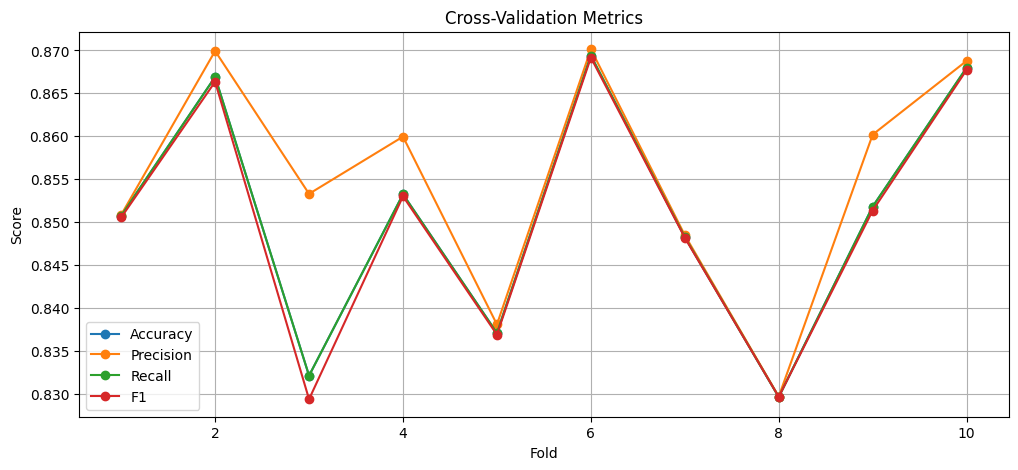
\includegraphics[width=1\linewidth]{Images/9.png}
\caption{Cross-Validation Metrics Across Folds}
\label{fig:cross_validation}
\end{figure}

\subsection{Comparison with Other Models}

The performance of the proposed \textbf{DeepNeuroPred} model is compared with two state-of-the-art models: \textit{PredNeuroP} and \textit{NeuroPred-FRL}. Table~\ref{table:comparison} shows that \textbf{DeepNeuroPred} outperforms both models in key metrics, including \textit{accuracy}, \textit{precision}, \textit{recall}, and \textit{F1-score}. Specifically, it achieves an accuracy of 88.74\%, surpassing \textit{PredNeuroP} (86.40\%) and \textit{NeuroPred-FRL} (86.10\%), highlighting its superior ability to accurately classify neuropeptide sequences.

\begin{table}[h]
\centering
\renewcommand{\arraystretch}{1.5}
\begin{tabular}{lcccc}
\hline
\textbf{Method}      & \textbf{Accuracy} & \textbf{Precision} & \textbf{Recall} & \textbf{F1-Score} \\ \hline
PredNeuroP           & 86.40\%           & 93.50\%            & 78.20\%         & 85.20\%           \\
NeuroPred-FRL        & 86.10\%           & 96.00\%            & 75.70\%         & 84.70\%           \\
DeepNeuroPred (Proposed) & 88.74\%           & 90.12\%            & 86.05\%         & 89.02\%           \\ \hline
\end{tabular}
\vspace{.3em}
\caption{Comparison of Model Performance}
\label{table:comparison}
\end{table}

\vspace{-1em}
When considering \textit{precision}, \textit{NeuroPred-FRL} slightly outperforms \textit{DeepNeuroPred} with a score of 96.00\% compared to 90.12\%. However, \textbf{DeepNeuroPred} achieves the highest \textit{recall} of 86.05\%, indicating a better ability to identify positive instances, such as neuropeptides, with fewer false negatives. Additionally, \textit{DeepNeuroPred} has the highest \textit{F1-score} of 89.02\%, balancing precision and recall. These results highlight that DeepNeuroPred is not only more accurate but also superior in identifying and classifying neuropeptide sequences compared to \textit{PredNeuroP} and \textit{NeuroPred-FRL}.

\subsection{Visualization of Predictions using t-SNE}

To visualize how the model's embeddings are distributed across different classes, we used t-SNE (t-Distributed Stochastic Neighbor Embedding), a technique for reducing high-dimensional data to two dimensions. The scatter plot in Figure~\ref{fig:tsne_plot} shows the 2D embeddings generated by the \textit{DeepNeuroPred} model on the test data.

For each input, we calculated the mean embedding across the sequence length, which was then reduced to 2D using t-SNE. The resulting plot shows well-separated clusters for each class, indicating that the model effectively distinguishes between them. The clustering within each class further suggests that the embeddings capture relevant features of the input sequences.

\begin{figure}[h]
\centering
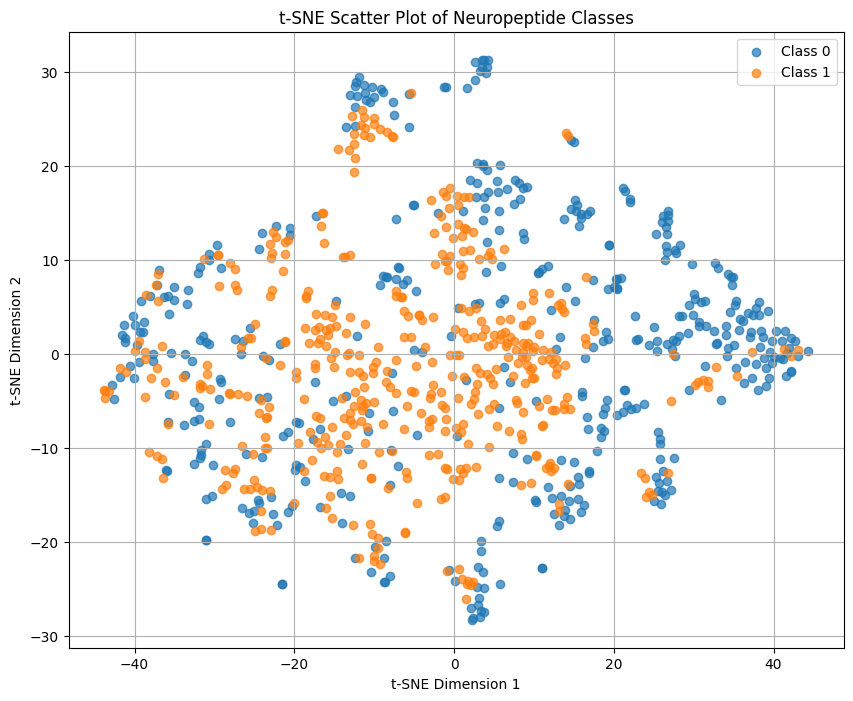
\includegraphics[width=0.5\textwidth]{Images/10.png}
\vspace{-.6em}
\caption{t-SNE Visualization of Neuropeptide Classes}
\label{fig:tsne_plot}
\end{figure}
\vspace{-.6em}
These results highlight the model's ability to learn meaningful representations for neuropeptide classification.

Additionally, we present a few sample predictions from the model:

\begin{itemize}
    \vspace{.3em}
    \item \textbf{Input:} K P S G F L G M R \\
    \textbf{Original Label:} 1 - \textbf{Predicted Label:} 1
    \item \textbf{Input:} M D D H H V W L E Q R L \\
    \textbf{Original Label:} 0 - \textbf{Predicted Label:} 0
    \item \textbf{Input:} M V N L A C E Q H I N I L H L Q H G N \\
    \textbf{Original Label:} 0 - \textbf{Predicted Label:} 0
    \item \textbf{Input:} K K I D T R T G K T M E K T E K K I E L S L K N M K T A T \\
    \textbf{Original Label:} 0 - \textbf{Predicted Label:} 0
    \vspace{.3em}
\end{itemize}

These examples show that the model accurately predicts the correct class labels, highlighting the effectiveness of the learned embeddings for classifying neuropeptide sequences. The model's ability to make precise and reliable predictions demonstrates its capability to differentiate between classes, validating its performance in neuropeptide classification.

\section{Conclusion}
This study introduces a novel classification model, \textbf{DeepNeuroPred}, for predicting neuropeptides, which outperforms traditional and current state-of-the-art methods in various performance metrics. The model achieved an impressive accuracy of \textbf{88.74\%}, with precision and recall scores of \textbf{90.12\%} and \textbf{86.05\%}, respectively. These results demonstrate the model's ability to effectively capture and classify complex sequence patterns while maintaining high interpretability. By employing tokenization techniques and leveraging a transformer-based architecture, \textit{DeepNeuroPred} addresses the inherent challenges in the neuropeptide classification domain, including sequence diversity, class imbalance, and interpretability. The model also integrates rigorous regularization techniques that contribute to its robustness and generalizability, ensuring that it remains effective even with varied data inputs.

Furthermore, the model offers valuable insights into the significance of sequence elements through its attention mechanisms, enhancing transparency and interpretability critical for bioinformatics and related fields. Its ability to efficiently process large-scale sequence data makes \textit{DeepNeuroPred} a promising tool for advancing neuropeptide prediction in biological research, especially in drug discovery, disease modeling, and synthetic biology.

\section{Future Scope}
While \textbf{DeepNeuroPred} has outperformed existing models in neuropeptide classification, there are several opportunities for further improvement:

\begin{itemize}
    \item \textbf{Exploring Alternative Architectures:} Exploring graph neural networks (GNNs) to better capture complex relationships between neuropeptide sequences and their receptors.
    
    \item \textbf{Incorporating Additional Biological Features:} Including structural properties, evolutionary data, or molecule interactions could enhance the model’s predictive power and interpretability.
    
    \item \textbf{Improving Accuracy:} Despite strong results, there is potential for achieving higher accuracy through further model refinement and experimentation with hyperparameters.
    
    \item \textbf{Developing a Software Program:} To make the model more accessible, we aim to develop a user-friendly software program for seamless neuropeptide classification in real-world applications.
\end{itemize}

\begin{thebibliography}{1}

\bibitem {meydan2013} C. Meydan, H. H. Otu, and O. U. Sezerman, ``Prediction of peptides binding to MHC class I and II alleles by temporal motif mining,'' \emph{BMC Bioinformatics}, vol. 14, Suppl 2, S13, 2013. https://doi.org/10.1186/1471-2105-14-S2-S13.

\bibitem {li2008} Z. C. Li, X. B. Zhou, Z. Dai, and X. Y. Zou, ``Prediction of protein structural classes by Chou’s pseudo amino acid composition: Approached using continuous wavelet transform and principal component analysis,'' \emph{Amino Acids}, vol. 37, pp. 415-425, 2008. https://doi.org/10.1007/s00726-008-0170-2.

\bibitem {salam2024} A. Salam, F. Ullah, F. Amin, I. A. Khan, E. Garcia Villena, A. K. Castilla, and I. de la Torre, ``Efficient prediction of anticancer peptides through deep learning,'' submitted April 29, 2024, accepted June 11, 2024, and published July 19, 2024.

\bibitem {yi2019} H. C. Yi, Z. H. You, X. Zhou, L. Cheng, X. Li, T. H. Jiang, and Z. H. Chen, ``ACP-DL: A Deep Learning Long Short-Term Memory Model to Predict Anticancer Peptides Using High-Efficiency Feature Representation,'' \emph{Mol Ther Nucleic Acids}, vol. 17, pp. 1-9, Sept. 2019. doi: 10.1016/j.omtn.2019.04.025. PMID: 31173946; PMCID: PMC6554234.

\bibitem {rives2021} A. Rives, J. Meier, T. Sercu, and R. Fergus, ``Biological structure and function emerge from scaling unsupervised learning to 250 million protein sequences,'' \emph{Proceedings of the National Academy of Sciences}, vol. 118, no. 15, e2016239118, 2021. https://doi.org/10.1073/pnas.2016239118.

\bibitem {elnaggar2021} A. Elnaggar, M. Heinzinger, C. Dallago, G. Rihawi, Y. Wang, L. Jones, T. Gibbs, T. Feher, C. Angerer, M. Steinegger, D. Bhowmik, and B. Rost, ``ProtTrans: Towards Cracking the Language of Life's Code Through Self-Supervised Deep Learning and High Performance Computing,'' arXiv, July 13, 2020, last revised May 4, 2021. arXiv:2007.06225v3 [cs.LG].

\bibitem {li2024} H. Li, L. Jiang, K. Yang, S. Shang, M. Li, and Z. Lv, ``iNP\_ESM: Neuropeptide Identification Based on Evolutionary Scale Modeling and Unified Representation Embedding Features,'' \emph{International Journal of Molecular Sciences}, vol. 25, no. 13, article 7049, 2024. https://doi.org/10.3390/ijms25137049.

\bibitem{wang2023} L. Wang, C. Huang, M. Wang, Z. Xue, Y. Wang, ``NeuroPred-PLM: an interpretable and robust model for neuropeptide prediction by protein language model,'' \emph{Briefings in Bioinformatics}, vol. 24, no. 2, bbad077, Mar. 2023. https://doi.org/10.1093/bib/bbad077

\end{thebibliography}

\smallskip
\end{document}